\section{Dynamisch modelleren: toestands- en activiteiten diagrammen}


Naast de tot hiertoe beschreven diagrammen die een puur statisch beeld geven van het systeem en aantonen hoe een aantal dingen in verband staan tot elkaar, zijn er ook diagrammen nodig om het dynamische gedrag voor te stellen en aantonen hoe de dingen samenwerken. Dit dynamische gedrag treedt op een specifiek moment in de levensloop van een systeem op, verandert in de tijd en bevat complexe interacties tussen objecten door het versturen van berichten. Dit betekent concreet dat operaties aangeroepen worden. In UML wordt dit met een aantal diagrammen beschreven:

\begin{itemize}
    \item toestandsdiagrammen beschrijven welke toestanden een object tijdens zijn levenscyclus kan hebben
    \item activiteitendiagrammen geven de interactie weer met de nadruk op het werk
    \item sequentiediagrammen beschrijven hoe objecten onderling samenwerken, met nadruk op het tijdsaspect
    \item collaboratiediagrammen beschrijven ook hoe objecten samen werken maar met de nadruk op ruimte in plaats van tijd.
\end{itemize}


\subsection{Concepten van het toestandsdiagram}

Het toestandsdiagram is in feite een aanvulling bij de beschrijving van een klasse. Het beschrijft de levenscyclus van een object. 

Het toont alle mogelijke toestanden waarin een object van deze klasse zich kan bevinden, met daarbij ook de gebeurtenissen (events) die kunnen leiden tot een verandering naar een andere toestand. Zo'n verandering van \textcolor{red}{toestand wordt ook een transitie (toestandsovergang)} genoemd. 

Toestandsdiagrammen worden niet getekend voor alle klassen, maar alleen voor die klassen die over een aantal duidelijk te beschrijven toestanden beschikken, of die met andere woorden een dynamisch gedrag vertonen. 

Mogelijks gebruikte synoniemen zijn: state chart, state machine


\subsubsection{toestand}

elk object bevindt zich in een bepaalde toestand die bepaald wordt door eerder uitgevoerde activiteiten en door de waarden van zijn attributen en eventuele links naar andere objecten.

%afbeelding nog plaatsen

\begin{center}
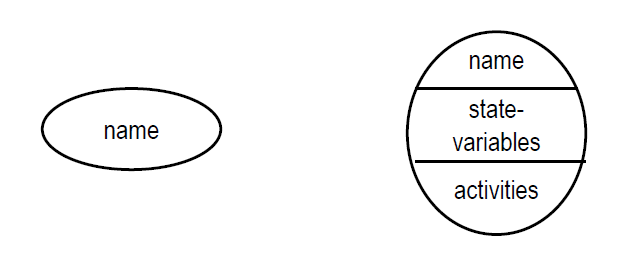
\includegraphics[width=4in]{img/state2}%
\end{center}

Een toestand kan 3 compartimenten hebben:

1) het eerste compartiment toont de naam van de toestand, 

2) het tweede compartiment is optioneel en kan de toestandsvariabelen bevatten (hierin kunnen variabelen geplaatst en toegekend worden) 

3)en het derde compartiment is ook optioneel en bevat de opsomming van acties en activiteiten.

Toestandsvariabelen kunnen bijvoorbeeld een timer zijn, waarbij een activiteit dan de waarde van die timer in de gaten houdt. Of een teller die het aantal pogingen bijhoudt, bijvoorbeeld om bij te houden datje maximaal 3 pogingen krijgt om een wachtwoord correct in te tikken.

Activiteiten bestaan uit \textbf{gebeurtenissen} en \textbf{acties}. 

Drie veelgebruikte zijn: 

- entry (wat gebeurt als het object in deze toestand terecht komt), 
- exit (wat gebeurt er als het object de toestand verlaat) 
- do (wat gebeurt er zolang het object in deze toestand is).

Het is belangrijk om het onderscheid te maken tussen events (gebeurtenissen) en toestanden. 

Een toestand is \textbf{stabiel} en heeft een \textbf{bepaalde tijdsduur} (bijvoorbeeld slapen), 

terwijl een event (gebeurtenis) iets is \textbf{zonder tijdsduur} en dat een \textbf{verandering tot gevolg heeft} (bijvoorbeeld in slaap vallen: het kan een tijd geduurd hebben voor het lukte, maar het in slaap vallen zelf heeft geen tijdsduur).

\subsubsection{transitie}

Een object kan door bepaalde events (gebeurtenissen) veranderen van toestand. Dan wordt gesproken over \textbf{transitie}.

%afbeelding nog plaatsen

\begin{center}
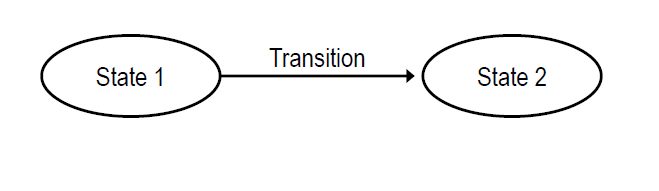
\includegraphics[width=4in]{img/state1}%
\end{center}

\subsubsection{Begin- en eindtoestand}

Elk toestandsdiagram heeft een beginpunt (de initiële toestand) en kan 0, 1 of meerdere eindpunten hebben.

Het beginpunt geeft aan in welke toestand het object terecht komt nadat het gecreëerd werd en wordt voorgesteld door een gevulde cirkel.

Het eindpunt geeft aan wanneer en hoe het object vernietigd wordt en wordt voorgesteld door een bull's eye (gevulde cirkel met een cirkel eromheen).

%afbeelding nog plaatsen

\begin{center}
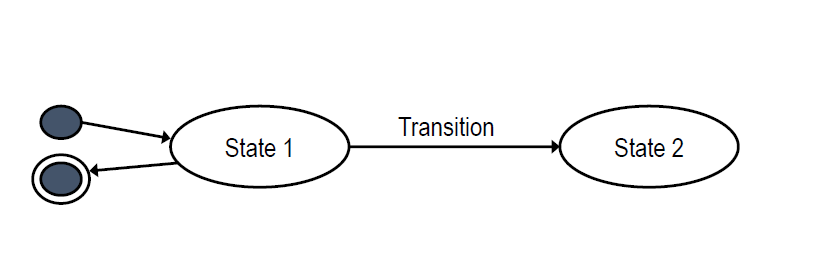
\includegraphics[width=4in]{img/state3}%
\end{center}

\subsubsection{Gebeurtenis (event)}

Een gebeurtenis is iets wat zich voordoet in de reële wereld en dat er de oorzaak van is dat er een transitie optreedt. 

Het heeft bovendien \textbf{geen tijdsduur}.

Hierdoor zal het object veranderen van toestand. 

Dit kan een voorwaarde zijn die op een bepaald moment voldaan wordt, of de ontvangst van een signaal van een ander object, of de ontvangst van een oproep voor een bepaalde operatie, of het verloop van een bepaalde tijdsspanne.

\textit{\textbf{Voorbeeld.}} Als een alarm in toestand 'wakend' is en een signaal opvangt van een mogelijke inbreker, verandert de toestand van 'wakend' naar 'bellend'.

\subsubsection{Actie}

Een actie beschrijft wat er moet gebeuren als de transitie zich voordoet. 

Het stelt dus een neveneffect voor bij de transitie. 

Een actie is altijd een \textbf{atomaire operatie} en kan dus niet onderbroken worden.

Voorbeeld. Als in het alarm het signaal van een inbreker opgevangen wordt, moet de geluidsinstallatie opgezet worden. Dit is dan een actie die ondernomen wordt bij de transitieverandering.

\subsubsection{Zelftransitie}

Een zelftransitie doet zich voor als een object door een bepaalde transitie in dezelfde toestand terecht komt als deze waarin hij zich bevond voor de transitie zich voordeed.

%afbeelding nog plaatsen

\begin{center}
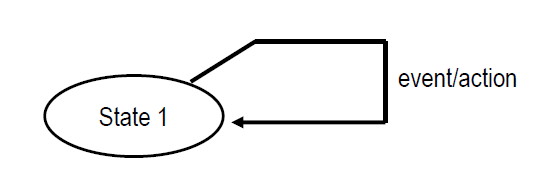
\includegraphics[width=4in]{img/state4}%
\end{center}

\subsubsection{Automatische transitie}

Een automatische transitie doet zich voor als een object verandert van toestand zonder dat zich daarom een bepaalde gebeurtenis voorgedaan heeft. Daardoor wordt het ook dikwijls een \textbf{triggerloze transitie} genoemd.

Dit kan zich voordoen als bijvoorbeeld een bepaalde activiteit afgerond is, of als een bepaalde voorwaarde voldaan wordt.

%afbeelding nog plaatsen

\begin{center}
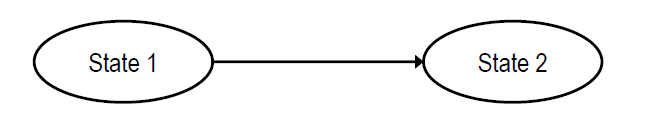
\includegraphics[width=4in]{img/state5}%
\end{center}

\subsubsection{Bewakingsvoorwaarde (guard)}

Een guard is een voorwaarde die aangegeven wordt en voldaan moet zijn voor de transitie zich kan voordoen. 

Deze kan gepaard gaan met een event, maar kan ook alleen staan. Op het moment dat deze \textbf{voorwaarde voldaan} is, zullen we dus een \textbf{automatische transitie} hebben.

%afbeelding nog plaatsen

\begin{center}
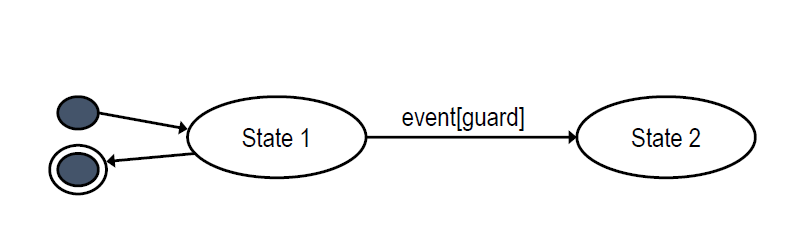
\includegraphics[width=4in]{img/state6}%
\end{center}

\subsubsection{Subtoestand}

Subtoestanden laten toe dat er een zeker niveau is van nesting. 

Op die manier kunnen een aantal toestanden beschouwd worden als een toestand op hoger niveau.

%afbeelding nog plaatsen

\begin{center}
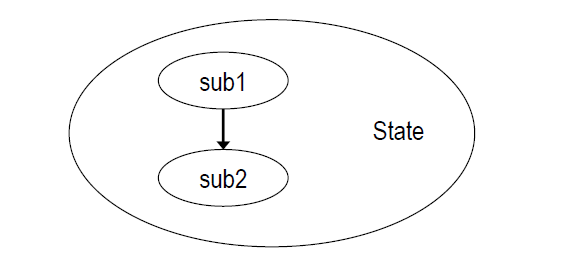
\includegraphics[width=4in]{img/substate}%
\end{center}

Op deze manier kunnen transities getekend worden vanuit de subtoestanden naar andere (al dan niet binnen dezelfde supertoestand), alsook vanuit de supertoestand naar andere toestanden.

\textbf{Sequentiële toestanden}= Sequentiële subtoestanden volgen elkaar op

\textbf{Gelijktijdige toestanden}: 
Zoals de naam het zegt, doen gelijktijdige toestanden zich gelijktijdig voor. Deze gelijktijdigheid wordt voorgesteld door een stippellijn in de supertoestand die de gelijktijdige toestanden van elkaar onderscheidt.

\subsubsection{Compositietoestand}

Als bij subtoestanden \textbf{elke toestand slechts deel is van één geheel}, dan heb je te maken met een compositietoestand. Dit kan een beetje vergeleken worden met composities zoals die besproken werden bij klassendiagrammen.

\subsubsection{Historietoestand}

Als een compositietoestand moet onthouden wat de actieve subtoestand was alvorens deze compositietoestand te verlaten, wordt gebruik gemaakt van een historietoestand.

Deze wordt aangeduid door een letter H omsloten door een cirkel en verbonden door een ononderbroken lijn met de subtoestand die onthouden moet worden.

De historietoestand en de initiële toestand (gevulde cirkel die aangeeft welke toestand de begintoestand is) zijn \textbf{pseudotoestanden} omdat ze geen echte toestanden voorstellen en niet volledig zijn aangezien ze nooit toestandsvariabelen en activiteiten kunnen hebben.

\subsubsection{Bericht}

Objecten communiceren door berichten naar elkaar te versturen. Ais dit bericht een operatieoproep in een ander object teweeg brengt kan dit in het toestandsdiagram aangeduid worden door de naam te laten voorafgaan door een pijlpunt.

\subsubsection{Signaal}

Een bericht dat een transitie in het toestandsdiagram van een ander object triggert, wordt een signaal genoemd. Dit kan ook een signaal zijn dat vanuit de buitenwereld komt.

\subsection{Toestandsdiagram: werkwijze}

De hieronder aangegeven stappen moeten uitgevoerd worden voor elke dynamische klasse in het klassendiagram.

\begin{itemize}
    \item Vind de mogelijke toestanden van een object van deze klasse
    
    Voor elke klasse wordt nagegaan wat de verschillende toestanden zijn waarin een object van deze klasse zich kan bevinden. Hierbij wordt ook al gecontroleerd welke events daarbij komen kijken. Deze kunnen in het toestandsdiagram getekend worden.
    \item Vind voor elke toestand de bijhorende transities
    
    Hier worden alle nodige pijlen getekend in het toestandsdiagram. Er wordt met andere woorden aangegeven waardoor het object van toestand kan veranderen.
    \item Voeg begin- en eindtoestanden toe
    
    Controleer in welke toestand het object terecht komt bij creatie en teken dit in het diagram. Ga ook na wanneer een object vernietigd wordt en teken de eindtoestanden.
    \item Voeg acties toe
    
    Kijk of er bij de transities zich bepaalde neveneffecten kunnen voordoen.
    \item Voeg activiteiten toe
    
    Kijk of het object in bepaalde toestand bepaalde activiteiten uitvoert.
    \item Voeg bijkomende informatie toe
    
    Kijk of het toestandsdiagram volledig is en of er bepaalde extra informatie toegevoegd moet worden. Dit kan bijvoorbeeld in de vorm van guards, subtoestanden aanduiden, enz.
    
    \item Itereer over de gedane stappen voor alle klassen van het klassendiagram
    
    Controleer of het diagram volledig is en itereer indien nodig om te vervolledigen.
\end{itemize}

\subsection{ Terugkoppeling naar klassendiagram}

Voor elke dynamische klasse (dit is een klasse waarvoor een toestandsdiagram gemaakt werd) moet een extra attribuut toegevoegd worden aan de klasse. Dit attribuut is een toestandsvariabele van een string-datatype en bevat de waarde van de toestand waarbinnen het object zich bevindt.
Daarenboven moeten alle events en transities die aangeduid zijn in het toestandsdiagram ook opgenomen worden als operatie in de desbetreffende klasse.

\subsection{ Het activiteitendiagram}

Het activiteitendiagram is feitelijk een variant op het toestandsdiagram, maar toont een stroom van activiteiten in plaats van de toestanden waarin een object zich kan bevinden. Het diagram bestaat uit actietoestanden die een specificatie bevatten van een uit te voeren activiteiten en taken. Een actietoestand verlaat de toestand op het moment dat de activiteit volledig is uitgevoerd.

Het activiteitendiagram toont de stappen die genomen moeten worden in een operatie of een proces en lijkt hiermee heel erg op de stroomschema's van vroeger.

Het activiteitendiagram wordt vooral gebruikt om \textbf{workflow management} voor te stellen. Het is een veel gebruikte manier om werkstromen te modelleren.

\subsection{ Concepten van het activiteitendiagram}

In een activiteitendiagram kunnen de volgende concepten onderscheiden worden:

\subsubsection{Activiteit}

Een activiteit stelt een reeks operaties voor die uitgevoerd moeten worden. Als de activiteit volledig uitgevoerd is, vindt een automatische transitie plaats. De verwerking vindt volledig plaats binnen de activiteit en daarna vindt een automatische transitie plaats.

%afbeelding nog plaatsen

\begin{center}
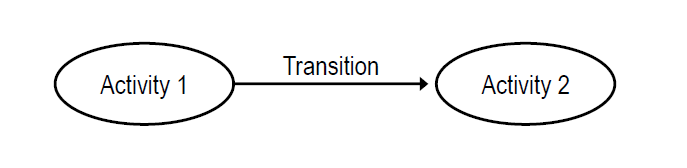
\includegraphics[width=4in]{img/activity1}%
\end{center}

\subsubsection{Transitie}

De transitie bestaat erin dat een activiteit volledig uitgevoerd is en aldus een overdracht van gegevens moet plaats vinden naar de volgende activiteitstoestand.

\subsubsection{Begin- en eindtoestand}

Ook in een activiteitendiagram heeft men juist 1 begintoestand en één of meerdere eindtoestanden. In tegenstelling met een toestandsdiagram MOET elk proces een eindtoestand hebben.

%afbeelding nog plaatsen

\begin{center}
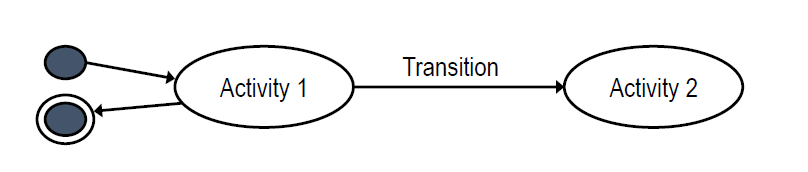
\includegraphics[width=4in]{img/activity2}%
\end{center}

\subsubsection{Beslissingen}

Een reeks activiteiten komt bijna altijd op een punt waar een beslissing moet plaats vinden. Het ene stel voorwaarden leidt naar het ene pad, het andere stel voorwaarden naar het andere. Beide paden sluiten elkaar uit.

%afbeelding nog plaatsen

\begin{center}
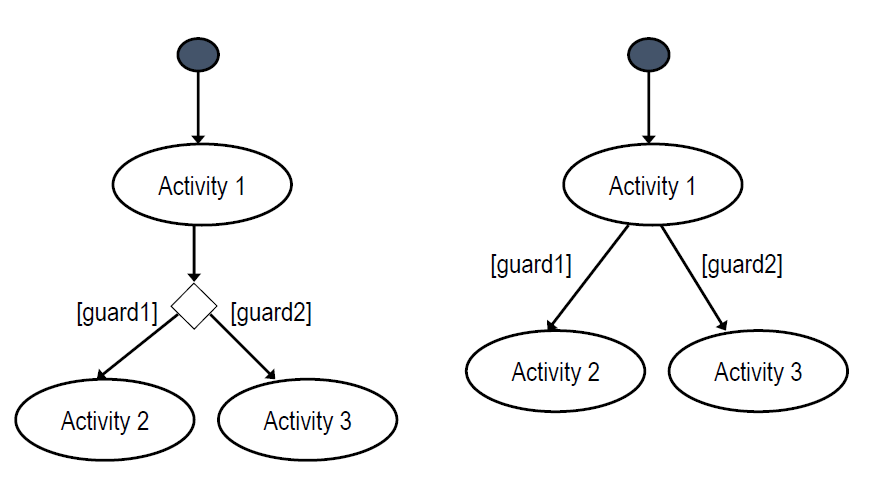
\includegraphics[width=4in]{img/decision3}%
\end{center}

\subsubsection{Gelijktijdige paden (parallellisme)}

Bij het modelleren van activiteiten is er de mogelijkheid om een transitie op te splitsen in 2 afzonderlijke paden die tegelijkertijd doorlopen worden en daarna weer samen komen.

%afbeelding nog plaatsen

\begin{center}
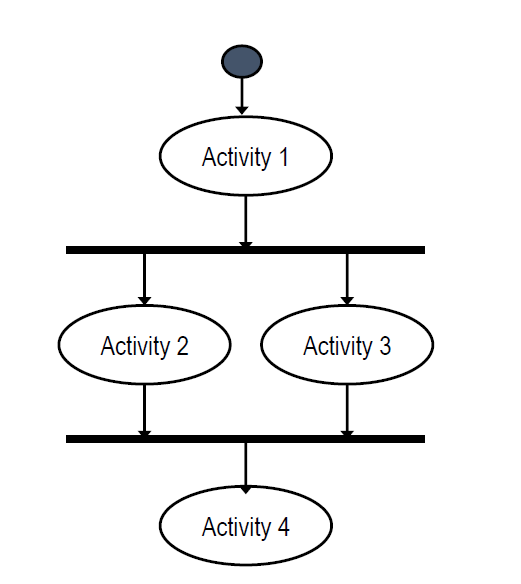
\includegraphics[width=4in]{img/parallelism}%
\end{center}

Voor het weergeven van de splitsing wordt een ononderbroken lijn loodrecht op de transitie gebruikt en worden paden getekend die uit de lijn komen. Het samenkomen van de paden wordt weergegeven door de paden naar een tweede ononderbroken lijn te laten wijzen.

\subsubsection{Signalen}

Tijdens een reeks activiteiten is het mogelijk een signaal te versturen. Als een signaal ontvangen wordt, veroorzaakt de ontvangst ervan een activiteit.
Het symbool voor het verzenden van een signaal is een vijfhoek waarvan één van de hoeken naar buiten steekt. Het symbool voor het ontvangen van een signaal is hetzelfde symbool, maar waarbij één van de hoeken naar binnen gericht is.

%afbeelding nog plaatsen

\begin{center}
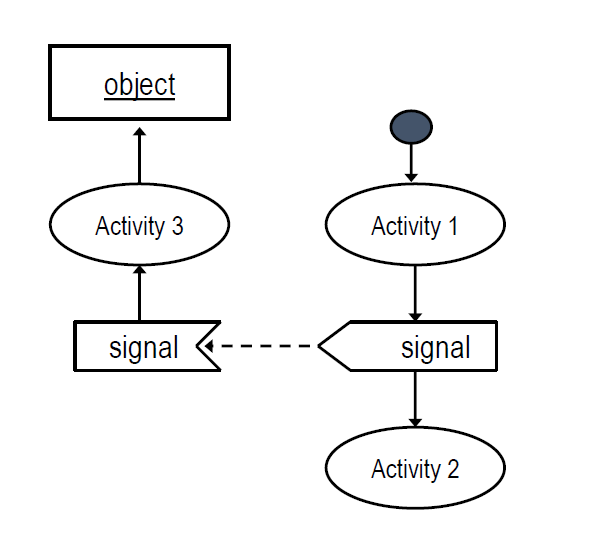
\includegraphics[width=4in]{img/signals}%
\end{center}

\subsubsubsection{Zwemlanen (swimlanes)}

Met behulp van zwemlanen kan in een activiteitendiagram aangeduid worden wie de verantwoordelijkheid heeft over de activiteiten in een activiteitendiagram. 

Deze verantwoordelijkheid kan voor elke activiteit apart aangeduid worden. 

Op deze manier kunnen rollen gevisualiseerd worden.

%afbeelding nog plaatsen

\begin{center}
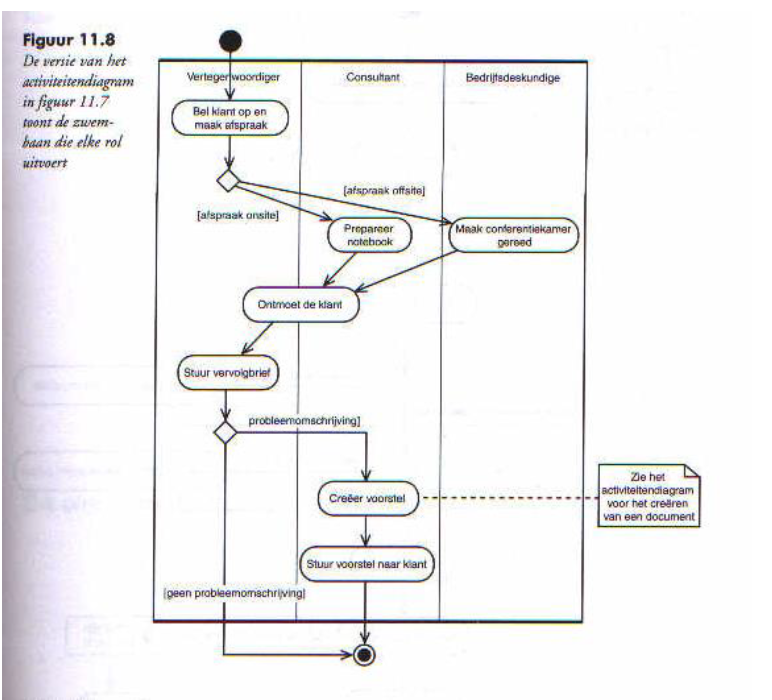
\includegraphics[width=4in]{img/swimlanes}%
\end{center}

\subsubsection{Hybride diagrammen}

In een hybride diagram kunnen symbolen uit verschillende soorten diagrammen gebruikt worden. Deze verschillende soorten symbolen kunnen met elkaar verenigd worden in één diagram.

%afbeelding nog plaatsen


\begin{center}
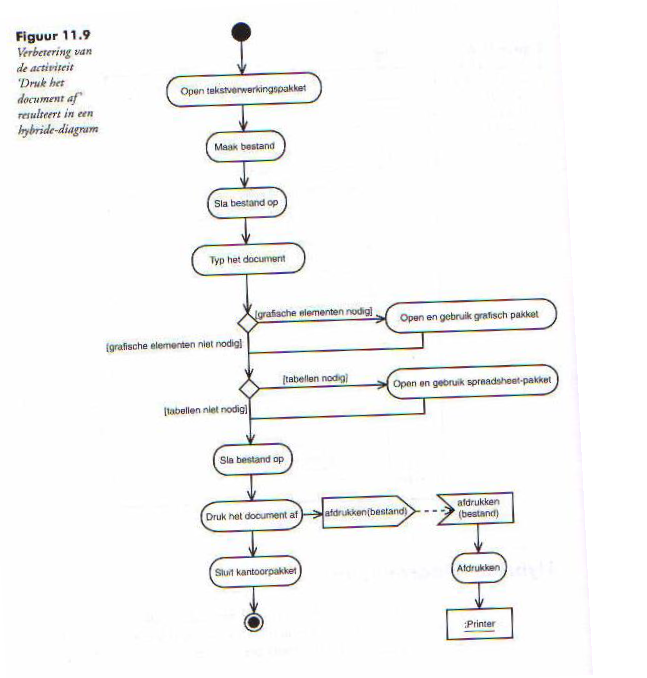
\includegraphics[width=4in]{img/hybride}%
\end{center}


